\documentclass[]{article}

%opening
\title{4F13 Probabilistic Machine Learning - Gaussian Processes}
\author{Lawrence Tray \\ St John's College}

%packages
\usepackage[margin=0.5in]{geometry}
\usepackage[export]{adjustbox}
\usepackage{graphicx}
\usepackage{amsmath}
\usepackage{amssymb}
\usepackage{hyperref}
\usepackage{caption}
\usepackage{subcaption}
\usepackage{parskip}
\usepackage{listings}
\usepackage{pdfpages}

%package setup
\graphicspath{{./img/}}
\DeclareMathOperator*{\argmax}{arg\,max}
\DeclareMathOperator*{\argmin}{arg\,min}

%custom commands
\newcommand{\dft}{\mathcal{F}}
\newcommand{\idft}{\mathcal{F}^{-1}}
\newcommand{\Xcal}{\mathcal{X}}
\newcommand{\Ncal}{\mathcal{N}}
\newcommand{\cmplx}{\mathbb{C}}
\newcommand{\Lcal}{\mathcal{L}}
\newcommand{\figwidth}{0.6\linewidth}

%section numbering
\renewcommand{\thesubsection}{\thesection.\alph{subsection}}

\begin{document}

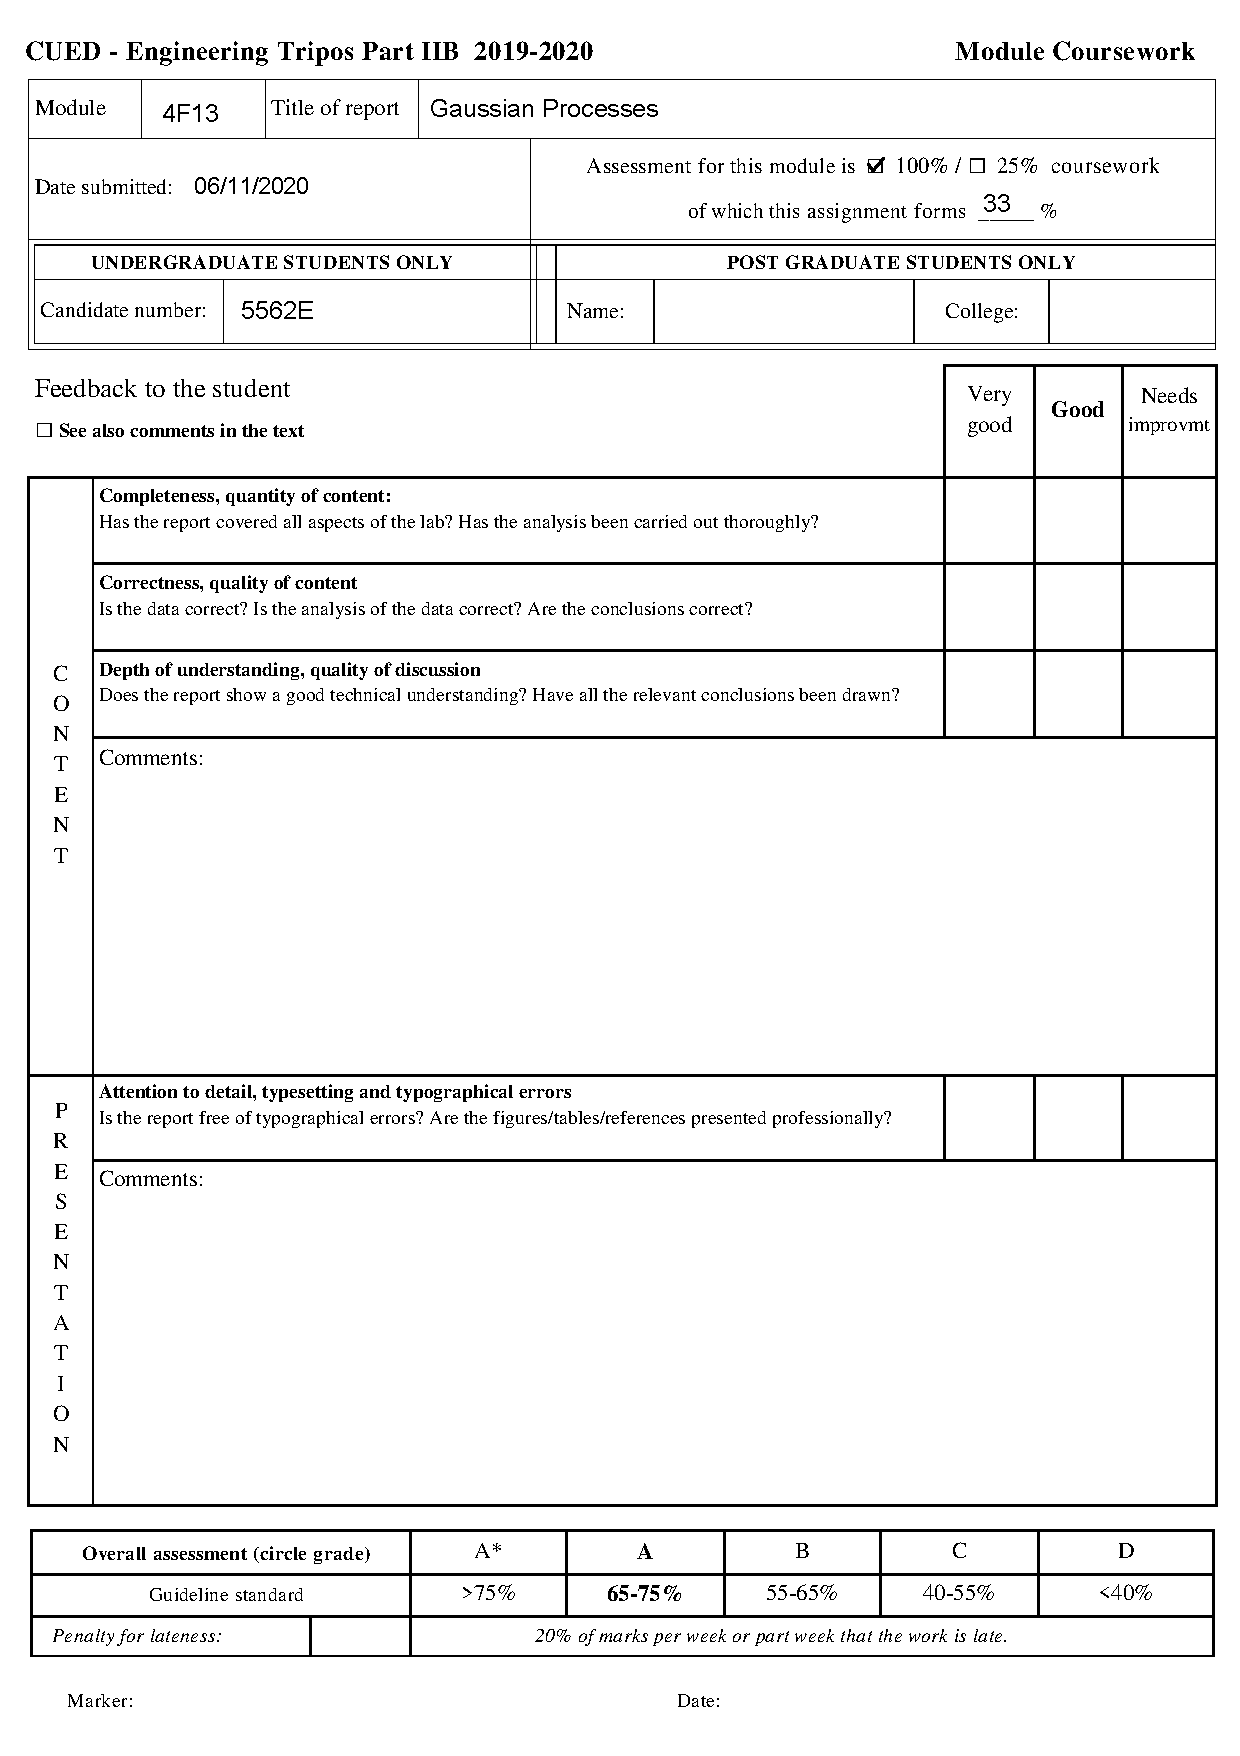
\includepdf[pages={1}]{coversheet.pdf}

\setcounter{page}{1}
\maketitle

\begin{abstract}
This report outlines the results of the first coursework for 4F13. Various properties of Gaussian Processes were investigated and how they can be used to model arbitrary data through careful choice of the covariance function. We focus on squared exponential (SE), periodic and composite combinations of these two covariance functions.
\end{abstract}

\tableofcontents

\section{Questions}
\subsection{Squared Exponential Covariance Function}

We start with the squared exponential (SE) covariance function (equation \ref{eqn:covSEiso}). For 1-D inputs this is necessarily isotropic.

\begin{equation}
k_{SE}(x, x') = \nu^2 \exp\left\{- \frac{(x-x')^2}{2\lambda^2}\right\}
\label{eqn:covSEiso}
\end{equation}

The hyperparameters are $\nu$ - scale factor and $\lambda$ - length scale. We load in the training data from \textit{`cw1a.mat'} and train a GP model, with zero mean and SE covariance. We assume a Gaussian likelihood function with noise variance $\sigma^2$ such that $P(y|\mu) = \Ncal(y; \mu, \sigma^2)$, where $\mu$ is the associated mean. We train the model hyperparameters by minimising the negative log marginal likelihood - denoted $\Lcal$. This is achieved through the commands in listing \ref{lst:opt}.

\begin{lstlisting}[frame=single, caption={Hyperparameter optimisation}, label={lst:opt}]
cov = [-1, 0]; lik = 0;
hyp = struct('mean', [], 'cov', cov, 'lik', lik);
hyp2 = minimize(hyp, @gp, -100, @infGaussLik, meanfunc, covfunc, likfunc, x, y);
\end{lstlisting}

\begin{table}[!h]
\centering
\begin{tabular}{c | c c | c c}
	\textbf{Parameter} & \textbf{A Initial} & \textbf{A Final} & \textbf{B Initial} & \textbf{B Final} \\ \hline
	$\log \lambda$           & -1                 & -2.054           & -0.45              & 2.085            \\
	$\lambda$                & 0.368              & 0.128            & 0.638              & 8.045            \\
	$\log \nu$         & 0                  & -0.109           & 0                  & -0.363           \\
	$\nu$              & 1                  & 0.897            & 1                  & 0.696            \\
	$\log \sigma$      & 0                  & -2.139           & 0                  & -0.411   \\
	$\sigma$           & 1                  & 0.118            & 1                  & 0.663    \\ \hline
	$\Lcal$            & 92.9               & 11.9             & 92.5               & 78.2  
\end{tabular}
\caption{Hyperparameter optimisation (log values included as reported by gpml toolbox)}
\label{tab:hyp-opt}
\end{table}

Table \ref{tab:hyp-opt} scenario A, shows one example of optimising the parameters\footnote{The negative log marginal likelihood $\Lcal$ is not a hyperparameter but rather a function evaluated on the dataset given the current setting of the hyperparameters. It is included in this table for reference.} to minimise the negative log-likelihood. This yields a predictor as in figure \ref{fig:1a}. The 95\% error bound is computed as within two standard deviations of the mean.

\begin{figure}[!h]
	\begin{subfigure}{0.5\linewidth}
		\centering
		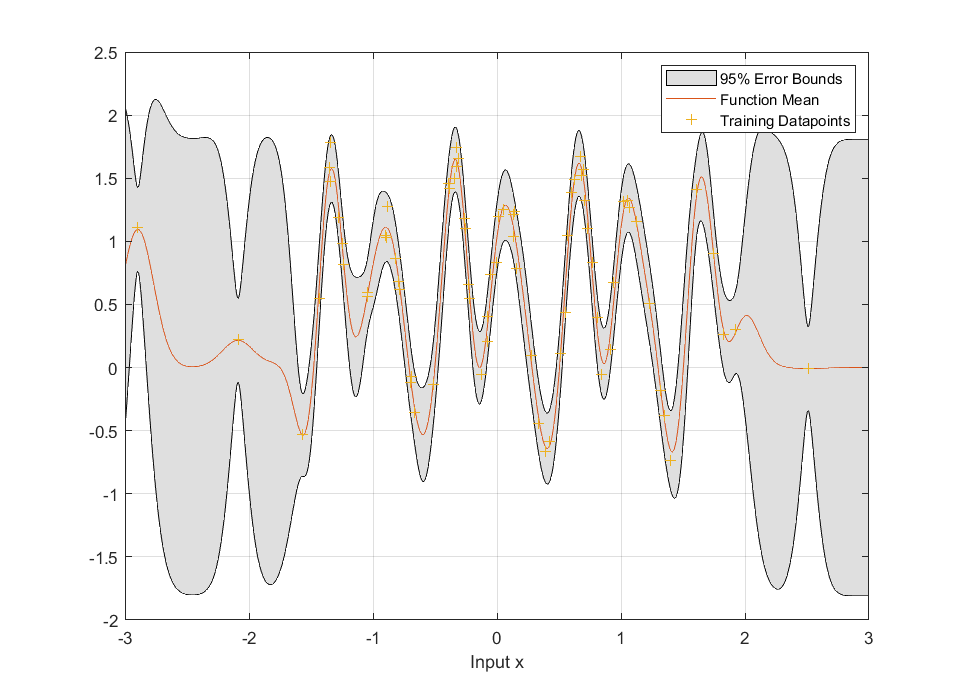
\includegraphics[width=\linewidth]{1a}
		\caption{Basic optimised hyperparameters (case A)}
		\label{fig:1a}
	\end{subfigure}
	\begin{subfigure}{0.5\linewidth}
		\centering
		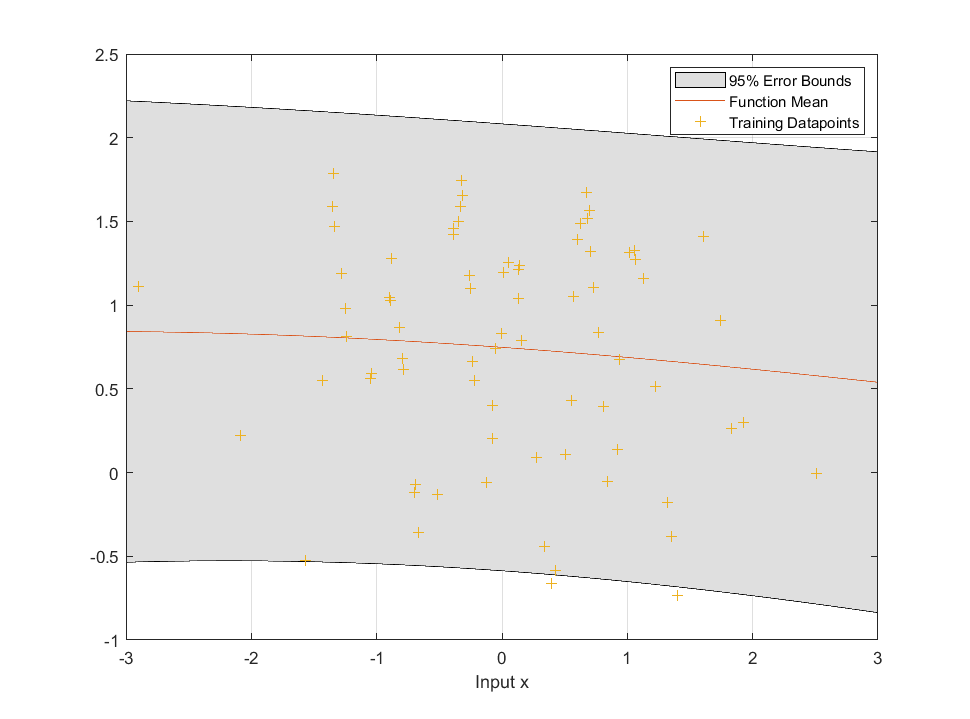
\includegraphics[width=\linewidth]{1b}
		\caption{Alternative optimised hyperparameter (case B)}
		\label{fig:1b}
	\end{subfigure}
	\caption{SE covariance GP trained on data from \textit{`cw1a.mat'}}
	\label{fig:1}
\end{figure}

We see that the error bars are small in regions of high data density; we cannot make confident predictions in areas of sparse data (e.g. $|x| \geq 2$).

We have that the length scale of variation $\lambda$ shrinks slightly to 0.128 - which agrees with the length scale of variation in the dataset. The model is able to match the data quite accurately. Indeed, the noise variance $\sigma$ shrinks significantly from 1 to 0.118 meaning the error bars are quite narrow in regions of high data density; the error bars remain large outside these regions due to the modest baseline variance $\nu=0.897$.

\subsection{Hyperparameter Initialisation}

However, the optimisation only finds a local minimum of the negative log-likelihood $\Lcal$. Therefore, a different initialisation of the hyperparameters can yield different results (case B of table \ref{tab:hyp-opt}). It was found that an initial value of $\log \lambda^{(0)} = -0.45$ was a critical point. Any setting of $\log \lambda^{(0)}$ above this would converge to the case-B optimum; anything below converges to the original case-A optimum. Varying $\nu^{(0)}$ only seemed to change the position of this critical point but would not converge to an altogether different solution.

This alternative optimum (B) converges to a very large value of the length scale $\lambda=8.045$. This expects data to vary very slowly with respect to $x$ and attributes all variation within the observed range to noise. Indeed, figure \ref{fig:1b} shows that the mean varies little over the data range. Parameter setting B does not seem to fit the data well just by comparing figures \ref{fig:1a} and \ref{fig:1b}. This intuition can be quantified through the marginal log-likelihood. Parameter setting B has a far larger final value of $\Lcal$, ($\Lcal_B=78.2 >> 11.9 = \Lcal_A$) so we can conclude that B is much more unlikely.


\subsection{Periodic Covariance Function}

We can instead use a periodic covariance function to model the data (as in equation \ref{eqn:covPeriodic}). We introduce a new parameter $\rho$, the period length. $\lambda$ should no longer be thought of as a length scale but rather sets the strength of the correlation between neighbours and $\nu$ scales the covariance. We tune the hyperparameters in the same way as before (results in table \ref{tab:per}).

\begin{equation}
k_{PER}(x, x') = \nu^2 \exp
\left\{
- \frac{2 \sin ^2 \left( \pi (x-x') / \rho \right)}{\lambda^2}
\right\}
\label{eqn:covPeriodic}
\end{equation}

\begin{table}[!h]
\centering
\begin{tabular}{c | c c}
	\textbf{Parameter} & \textbf{Initial} & \textbf{Final} \\ \hline
	$\log \lambda$     & 0                & 0.0437         \\
	$\lambda$          & 1                & 1.044          \\
	$\log \rho$        & 0                & -0.0012        \\
	$\rho$             & 1                & 0.999          \\
	$\log \nu$         & 0                & 0.2122         \\
	$\nu$              & 1                & 1.24           \\ 
	$\log \sigma$      & 0                & -2.213         \\
	$\sigma$           & 1                & 0.109          \\ \hline
	$\Lcal$            & 79.5             & -35.3
\end{tabular}
\caption{Periodic covariance function hyperparameter tuning}
\label{tab:per}
\end{table}

We plot the trained GP predictions on figure \ref{fig:1c} which shows excellent agreement between model and data. The error bars are uniformly small - even in regions of sparse data. This initially appears a better fit than the SE model. However, we must be careful to avoid overfitting.

\begin{figure}[!h]
	\begin{subfigure}{0.5\linewidth}
		\centering
		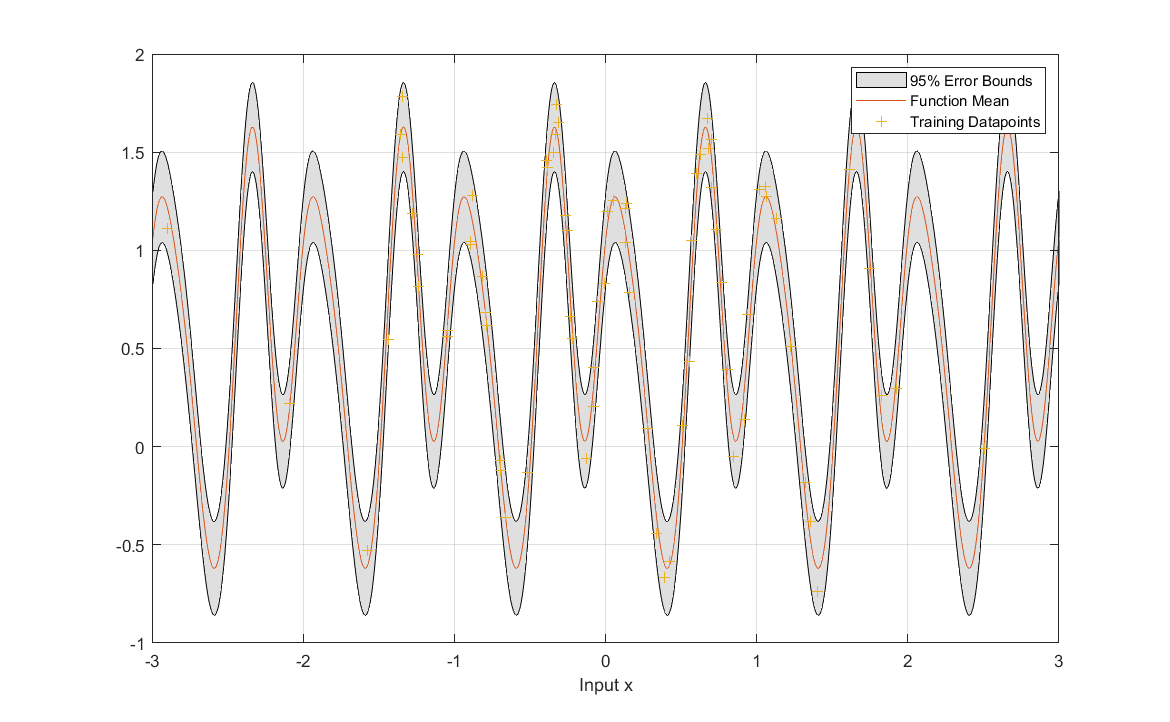
\includegraphics[width=\linewidth]{1c}
		\caption{Periodic covariance GP with tuned hyperparameters}
		\label{fig:1c}
	\end{subfigure}
	\begin{subfigure}{0.5\linewidth}
		\centering
		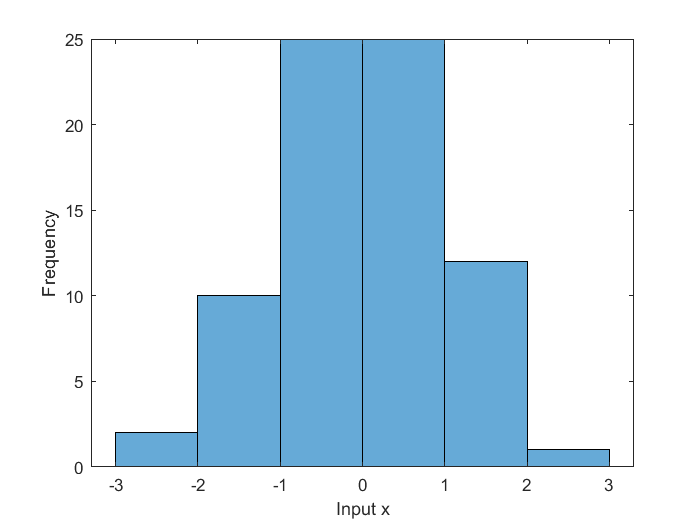
\includegraphics[width=\linewidth]{1c1}
		\caption{Histogram of training inputs}
		\label{fig:1c1}
	\end{subfigure}
	\caption{Periodic covariance fit on data from \textit{`cw1a.mat'}}
	\label{fig:1c-comb}
\end{figure}

Indeed, the log-likelihood is far larger for the periodic covariance model compared to the SE model. Nevertheless, it does not appear that the training data was generated in a periodic manner. On figure \ref{fig:1c1}, we plot a histogram of the training inputs. This appears Gaussian and not uniform. Therefore, it is highly unlikely that the data was generated by applying a periodic function to uniformly generated inputs across the range [-3, 3]. We prefer the model in part a (SE covariance) as this remains uncertain in areas of sparse data.


\subsection{Sampling from a Gaussian Process}

We can sample from an arbitrary GP at a finite array of input points $\mathbf{x}$, by evaluating the covariance matrix $K$ for these points and exploiting the Cholesky Decomposition ($\text{chol}(K) = C$ s.t. $C C^T = K$). The code for this is in listing \ref{lst:gp-sampling}. We must add a small diagonal matrix to ensure that $K$ is positive definite and thus accepts a Cholesky decomposition.

\begin{lstlisting}[frame=single, caption={GP sampling}, label={lst:gp-sampling}]
x = linspace(-5, 5, n)';
z = gpml_randn(seed, n, 1);
K = feval(covfunc{:}, cov, x);
K_pos_def = K + 1e-6 * eye(n);
y = chol(K_pos_def)'*z;
\end{lstlisting}

We use this code to sample from a GP with composite covariance function defined as the product of a periodic covariance function and a SE covariance function. The hyperparameters are set to $[\lambda, \rho, \nu]_{PER} = [0.607, 1, 1]$ for the periodic component and $[\lambda, \nu]_{SE} = [7.39, 1]$ for the SE component. We can run the code in \ref{lst:gp-sampling} for different values of the seed to yield the set of plots in figure \ref{fig:1d}.

\begin{figure}[!h]
	\begin{subfigure}{0.3\linewidth}
		\centering
		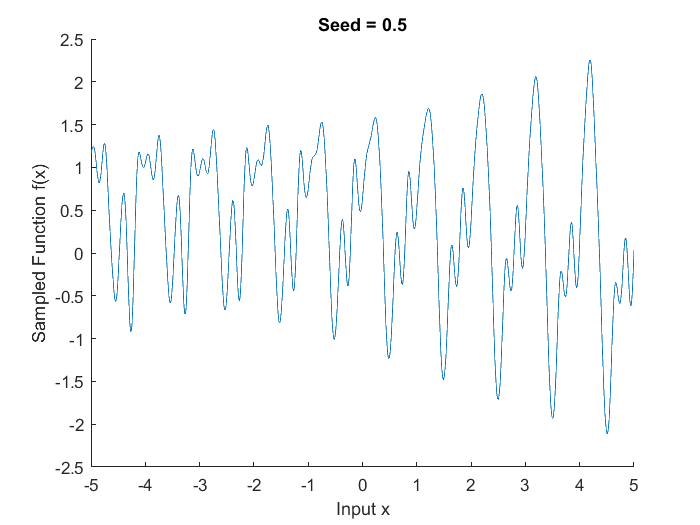
\includegraphics[width=\linewidth]{1d1}
		\caption{Seed = 0.5}
		\label{fig:1d1}
	\end{subfigure}
	\begin{subfigure}{0.3\linewidth}
		\centering
		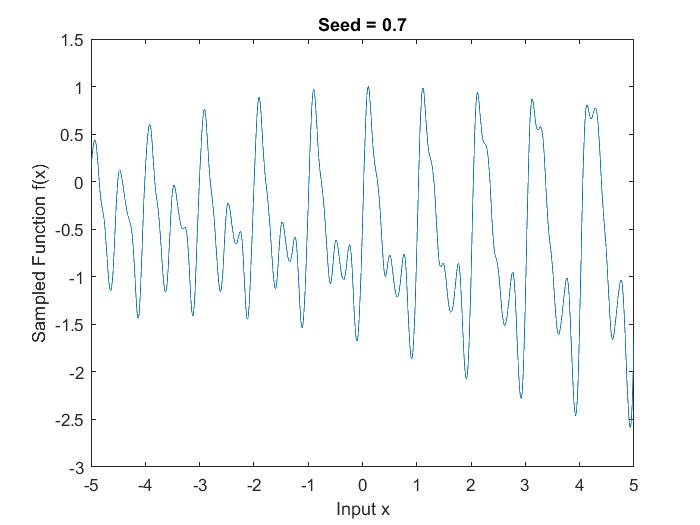
\includegraphics[width=\linewidth]{1d2}
		\caption{Seed = 0.7}
		\label{fig:1d2}
	\end{subfigure}
	\begin{subfigure}{0.3\linewidth}
		\centering
		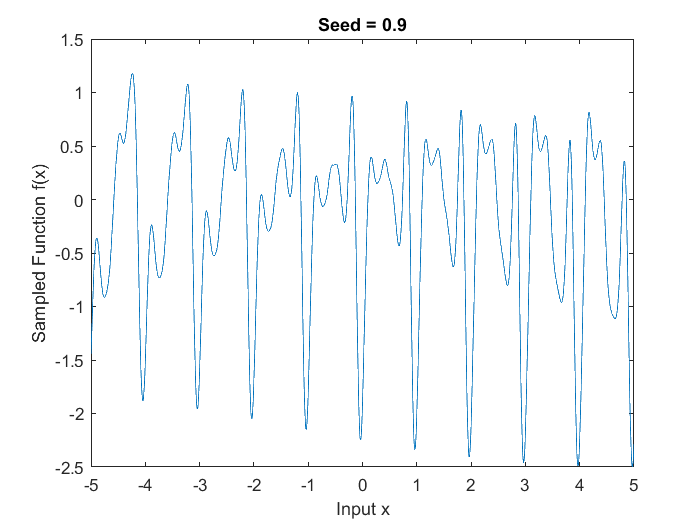
\includegraphics[width=\linewidth]{1d3}
		\caption{Seed = 0.9}
		\label{fig:1d3}
	\end{subfigure}
	\caption{Random function drawn from GP with composite product covariance: periodic $\times$ SE}
	\label{fig:1d}
\end{figure}

This set of characteristic functions share some key properties. The functions do appear in some way periodic with period 1. This agrees with the hyperparameter setting $\rho_{PER}=1$. The SE component has a very long length scale $\lambda_{SE}=7.39$ This means that we only see distortion of the periodic structure over long length scales; adjacent periods are very similar but those that are further apart have different form.

\subsection{2-Dimensional Input - Model Comparison}

We now extend our investigation to deal with 2-dimensional input data. For the simple case we choose a Squared Exponential - Automatic Relevance Determination (SE-ARD) covariance function. This is, in general, anisotropic - with formula given by equation \ref{eqn:covSEard}. The index $i$ iterates through every dimension in our input. Our data has $D=2$.

\begin{equation}
k_{ARD}(\mathbf{x}, \mathbf{x}') = \nu^2 \exp\left\{- \frac{1}{2} \sum_{i=1}^{D}\frac{(x_i-x_i')^2}{\lambda_i^2}\right\}
\label{eqn:covSEard}
\end{equation}

We wish to compare this simple model with a more complex, additive model. The covariance functions for the simple and additive model are given in equations \ref{eqn:cov-a} and \ref{eqn:cov-b}. The vector $\theta = [\nu, \lambda_1, \lambda_2]$ denotes the hyperparameters of the SE-ARD covariance function.

\begin{equation}
k^a(\mathbf{x}, \mathbf{x}') = k_{ARD}(\mathbf{x}, \mathbf{x}' ; \theta^a)
\label{eqn:cov-a}
\end{equation}
\begin{equation}
k^b(\mathbf{x}, \mathbf{x}') = k_{ARD}(\mathbf{x}, \mathbf{x}' ; \theta^{b1})
+ k_{ARD}(\mathbf{x}, \mathbf{x}' ; \theta^{b2})
\label{eqn:cov-b}
\end{equation}

The optimised parameters are presented in table \ref{tab:complex-opt}. We plot the mean of the predictive surface on figure \ref{fig:1e}. Both models fit the data quite well. Nevertheless, the additive model has a much lower $\Lcal$ and so matches the training data more closely. This is to be expected as model a is a special case of model b where $\nu^{(b2)}=0$. The additional degrees of freedom introduced by the more complex, additive model mean it can fit the data more closely and thus increases the marginal likelihood.

\begin{table}[!h]
	\centering
	\subfloat[Simple model a]{
		\begin{tabular}{c | c}
			\textbf{$\theta^a$} & \textbf{Final} \\ \hline
			$\log \lambda_1$            & 0.413          \\
			$\lambda_1$                 & 1.511          \\
			$\log \lambda_2$            & 0.252          \\
			$\lambda_2$                 & 1.287          \\
			$\log \nu$                  & 0.102          \\
			$\nu$                       & 1.107          \\
		\end{tabular}
	}
	\subfloat[Component b1]{
		\begin{tabular}{c | c}
			$\theta^{b1}$ & \textbf{Final} \\ \hline
			$\log \lambda_1$             & 0.3644         \\
			$\lambda_1$                  & 1.440          \\
			$\log \lambda_2$             & 6.3200         \\
			$\lambda_2$                  & 555.6          \\
			$\log \nu$                   & 0.0801         \\
			$\nu$                        & 1.083          \\
		\end{tabular}
	}
	\subfloat[Component b2]{
		\begin{tabular}{c | c c}
			$\theta^{b1}$ & \textbf{Final} \\ \hline
			$\log \lambda_1$              & 6.000          \\
			$\lambda_1$                   & 403.4          \\
			$\log \lambda_2$              & -0.0072        \\
			$\lambda_2$                   & 0.993          \\
			$\log \nu$                    & -0.3351        \\
			$\nu$                         & 0.715        
		\end{tabular}
	}
	\subfloat[Negative Log-likelihood]{
		\begin{tabular}{c | c c}
			 & \textbf{Model a}  & \textbf{Model b} \\ \hline
			$\Lcal$ & -19.2  & -66.3
		\end{tabular}
	}
	\caption{Parameter optimisation for 2-D data}
	\label{tab:complex-opt}
\end{table}

\begin{figure}[!h]
	\begin{subfigure}{0.5\linewidth}
		\centering
		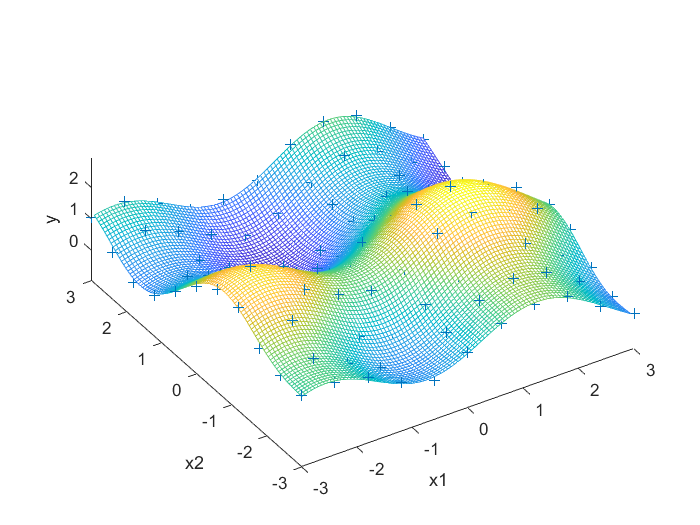
\includegraphics[width=\linewidth]{1e1}
		\caption{Basic covariance function}
		\label{fig:1e1}
	\end{subfigure}
	\begin{subfigure}{0.5\linewidth}
		\centering
		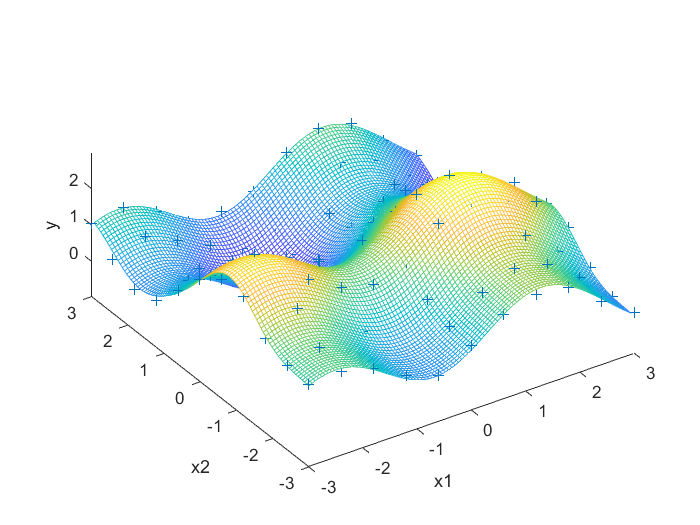
\includegraphics[width=\linewidth]{1e2}
		\caption{Additive covariance function}
		\label{fig:1e2}
	\end{subfigure}
	\caption{Comparison of covariance function fits on training data from \textit{`cw1e.mat'}}
	\label{fig:1e}
\end{figure}

Nevertheless, figure \ref{fig:1e} is hard to interpret so instead we plot the standard deviation surface of the trained GP's over the domain of interest (figure \ref{fig:std-dev}). For the simple model, the standard deviation surface (this is a measure of the uncertainty of each prediction) is approximately flat, only rising at the edges of the observed data. In particular the corners are highly uncertain as these have the fewest neighbouring data-points. The additive model has more ripples in its uncertainty surface due to its increased complexity. However, the magnitude of this uncertainty is uniformly lower.

\begin{figure}[!h]
	\begin{subfigure}{0.5\linewidth}
		\centering
		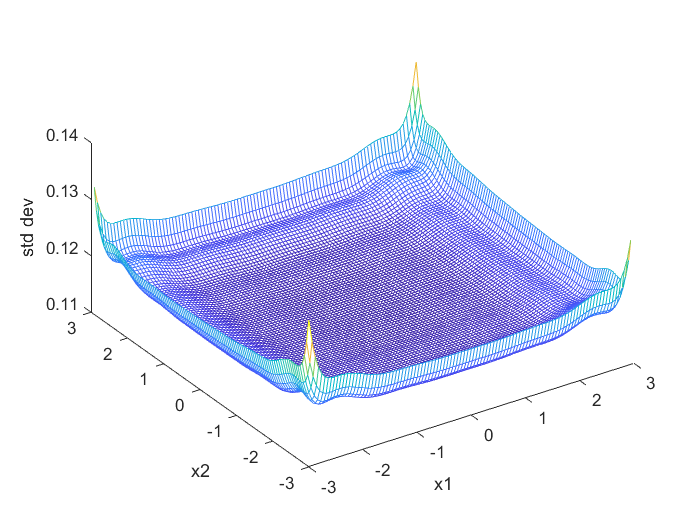
\includegraphics[width=\linewidth]{1e1b}
		\caption{Basic covariance function}
		\label{fig:1e1b}
	\end{subfigure}
	\begin{subfigure}{0.5\linewidth}
		\centering
		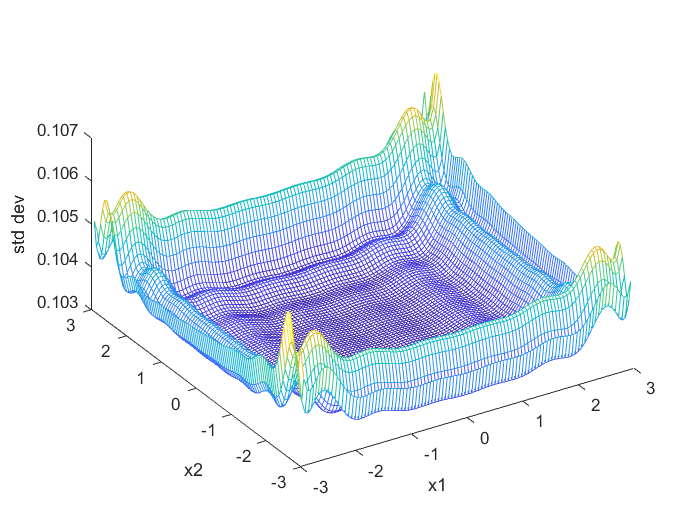
\includegraphics[width=\linewidth]{1e2b}
		\caption{Additive covariance function}
		\label{fig:1e2b}
	\end{subfigure}
	\caption{Comparison of standard deviation for the two models on \textit{`cw1e.mat'}}
	\label{fig:std-dev}
\end{figure}

\textbf{Words}: 987

\end{document}
